% Chapter 1 - Introduction
% Canonical MEIA structure: Contextualization, Problem, Research Questions & Objectives,
% Scientific Contributions, Document Structure. EN-GB. Every claim carries a verified source.

\chapter{Introduction}
\label{chap:introduction}

\section{Contextualization}
\label{sec:intro_context}

Most people in the United States now own stock. In 2025, 62\% of Americans reported holding shares,
either directly or through mutual funds and retirement accounts \autocite{gallup2025stock}, in a market
whose total value reached US\$62.2~trillion at the end of 2024, the largest and most liquid in the world
\autocite{sifma2025factbook}. Figure~\ref{fig:us_market_cap} shows how fast that market has grown, more
than doubling since 2015. Trading takes place mainly on two venues, the \gls{NYSE} and \gls{NASDAQ}, and
an increasing share of it now comes from ordinary people using commission-free mobile apps rather than
from professional institutions.

\begin{figure}[ht]
\centering
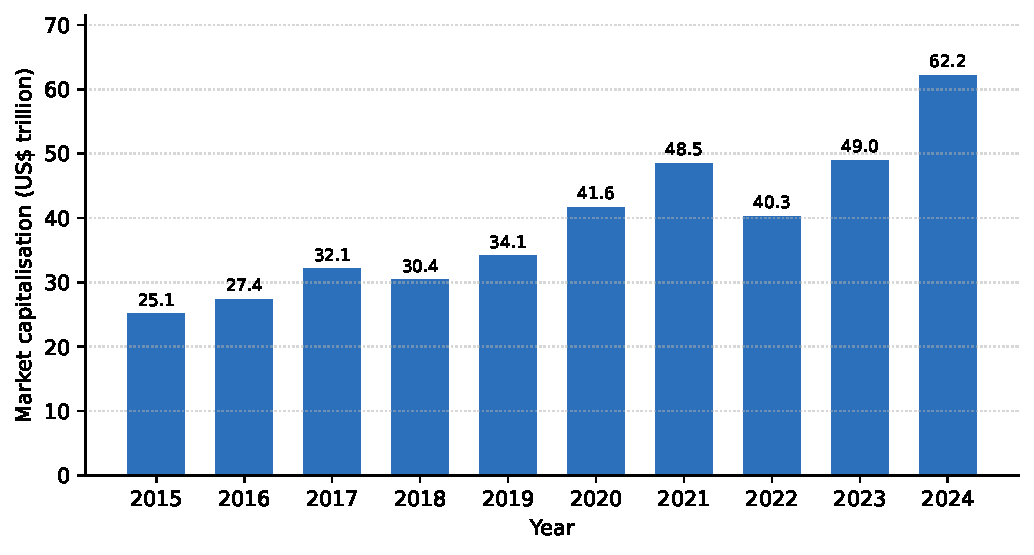
\includegraphics[width=0.9\textwidth]{figures/us_equity_market_cap.pdf}
\caption[US equity market capitalisation, 2015--2024]{US equity market capitalisation, 2015--2024
(US\$~trillion). Drawn from data reported in the SIFMA 2025 Capital Markets Fact Book
\autocite{sifma2025factbook}.}
\label{fig:us_market_cap}
\end{figure}

These non-professional, or ``retail'', investors are the audience of this work. Stock ownership among
them is wide but uneven: it rises to 87\% of households earning above US\$100{,}000 and falls to 28\%
below US\$50{,}000 \autocite{gallup2025stock}. What they share is a hard position. The market never stops
moving across thousands of stocks, financial news never stops arriving, and they have none of the tools
that banks and funds take for granted.

Artificial intelligence has, meanwhile, spread quickly through finance. A 2026 survey found that 81\% of
financial firms were adopting \gls{AI} in some form and 71\% were already using generative AI
\autocite{ccaf2026aifs}. Much of this technology is opaque: the strongest models rarely reveal how they
reach a conclusion \autocite{arrieta2020xai, adadi2018peeking}. For someone who has to act on an alert
and live with the result, that opacity is a real obstacle. Letting the investor see \emph{why} an alert
was raised is what this dissertation sets out to do.

\section{Problem Statement}
\label{sec:intro_problem}

A retail investor who wants to stay informed has two problems, not one. The first is telling a genuinely
unusual price move apart from ordinary daily volatility, which takes statistical judgement and constant
attention. The second is reading what a news item might mean, which takes knowledge of how similar events
played out in the past, knowledge most people do not have to hand. Consumer apps tend to make both
problems worse. They push alerts with no explanation, or they hide their reasoning inside a black box.

This work does not try to predict prices. It tries to \emph{explain}. For each abrupt move or relevant
news item, the system shows what it detected, how it reached that conclusion, where the information came
from, and which past events resemble the current one, alongside what happened to prices afterwards
(Figure~\ref{fig:concept}).

\begin{figure}[ht]
\centering
\begin{tikzpicture}[
  font=\small, >={Stealth[length=2.2mm]},
  trig/.style={draw, rounded corners, fill=black!8, align=center, text width=2.7cm, minimum height=0.9cm},
  sys/.style={draw, rounded corners, fill=black!3, align=center, text width=2.2cm, minimum height=1.4cm},
  outbox/.style={draw, rounded corners, fill=black!3, align=center, text width=3.4cm, minimum height=1.4cm},
]
  \node[trig] (t1) {Abrupt market move};
  \node[trig, below=6mm of t1] (t2) {Relevant news};
  \node[sys] (sys) at ($(t1)!0.5!(t2) + (3.6,0)$) {\textbf{CLARION}};
  \node[outbox, right=1.2cm of sys] (out) {Explained alert\\ \footnotesize event $\cdot$ reasoning\\ \footnotesize sources $\cdot$ precedents};
  \node[right=0.9cm of out] (inv) {\footnotesize investor};
  \draw[->] (t1) -- (sys);
  \draw[->] (t2) -- (sys);
  \draw[->] (sys) -- (out);
  \draw[->] (out) -- (inv);
\end{tikzpicture}
\caption[What CLARION does]{In one picture: two triggers --- a sudden market move or a relevant news item
--- feed CLARION, which replies not with a bare notification but with an explained alert that the
investor can follow and check.}
\label{fig:concept}
\end{figure}

\section{Research Questions and Objectives}
\label{sec:intro_objectives}

The aim is to design, build and evaluate an explainable financial-alert system for US retail investors,
driven by two independent triggers, a sudden market move and an incoming news item, and delivered over
Telegram. Three research questions guide the work:

\begin{itemize}
  \item \textbf{\gls{RQ}1.} Can transparent statistical methods detect abrupt market movements
        consistently enough to be useful to a retail investor, while staying explainable?
  \item \textbf{\gls{RQ}2.} Can a news--market correlation engine retrieve genuinely analogous historical
        news, and quantify its observed price impact without lookahead, better than trivial baselines?
  \item \textbf{\gls{RQ}3.} Can the resulting explanations be made faithful to what the system actually
        computes, and useful to a retail investor?
\end{itemize}

Four supporting objectives shape how the system is built: deliver a thin end-to-end slice first, so that
integration problems surface early; keep each component as simple as it can defensibly be; evaluate every
component against a plan fixed before any experiment is run; and make the whole system reproducible.

\section{Scientific Contributions}
\label{sec:intro_contributions}

This is a dissertation in Artificial Intelligence \emph{Engineering}. Its contribution is not a new
algorithm but the disciplined assembly of existing ones into a system that works, explains itself, and
can be reproduced. Three contributions stand out:

\begin{itemize}
  \item A reproducible method for relating news to market impact, pairing sentence-embedding retrieval
        with event-study windows, where the similarity measure and the time horizons are stated
        explicitly and no information about the future is allowed to leak in.
  \item \textbf{CLARION}, an alerting system whose whole reasoning chain --- the detected event, the
        evidence, the sources and the precedents --- is shown to a non-expert, and whose explanation is
        generated from the same quantities it computes, so the text and the computation cannot disagree.
  \item A critical evaluation of each core component on real data, against simple and lexical baselines,
        with the results, the ablations and the limitations all reported plainly.
\end{itemize}

\section{Document Structure}
\label{sec:intro_structure}

Chapter~\ref{chap:sota} reviews the state of the art behind the work: anomaly detection, explainable AI,
financial natural-language processing, event studies, and case-based reasoning. Chapter~\ref{chap:methods}
sets out the methods, the datasets and the evaluation design. Chapter~\ref{chap:clarion} presents CLARION
itself, at the level of its architecture and the decisions behind it. Chapter~\ref{chap:casestudies}
evaluates the system through three case studies on real data, and Chapter~\ref{chap:conclusions} returns
to the research questions, states what was and was not achieved, and points to future work.
